\clearpage  % move to another page
\begin{appendices}
\end{appendices}
\clearpage % move to another page

\chapter{Experiment Details}\label{chapter:experiment_details}

This appendix includes supplementary material for some of the experiments discussed in \autoref{chapter:experiments_and_results}.

\section{Intra-Class Feature Map Analysis}\label{appendix:s_bears_analysis}

This section analyzes the feature maps of the foreground objects in images of $C_{\text{bears}}$ (\autoref{fig:classes} (f-j)). The analysis process is identical to the process followed in \autoref{section:further_analysis}. 

We first rank the feature maps based on their $\Sigma$-scores (see \autoref{fig:barcharts2}). Then, we use parallel coordinates plots to visualize the distribution of the feature maps in the different clusters of the bears class (\autoref{fig:pcp_similar2} and \autoref{fig:pcp_dissimilar2}). Finally, we superimpose the five lowest- and highest-$\Sigma$-scoring feature maps on the original images (\autoref{fig:overlay_similar_dims2} and \autoref{fig:overlay_dissimilar_dims2}).

\begin{figure}[thbp]
    \centering
    \begin{subfigure}{.49\textwidth}
        \centering
        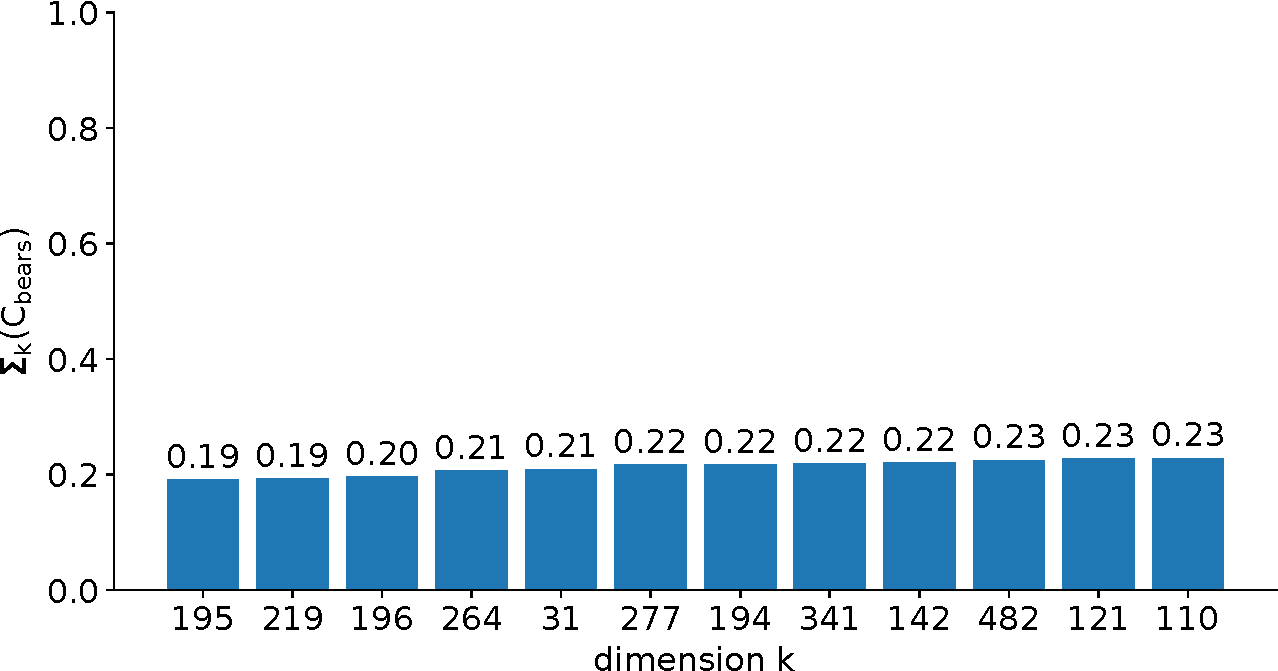
\includegraphics[width=\linewidth]{figures/lowest_scores_barchart_ds19.pdf}
    \end{subfigure}
    \hfill
    \begin{subfigure}{.49\textwidth}
        \centering
        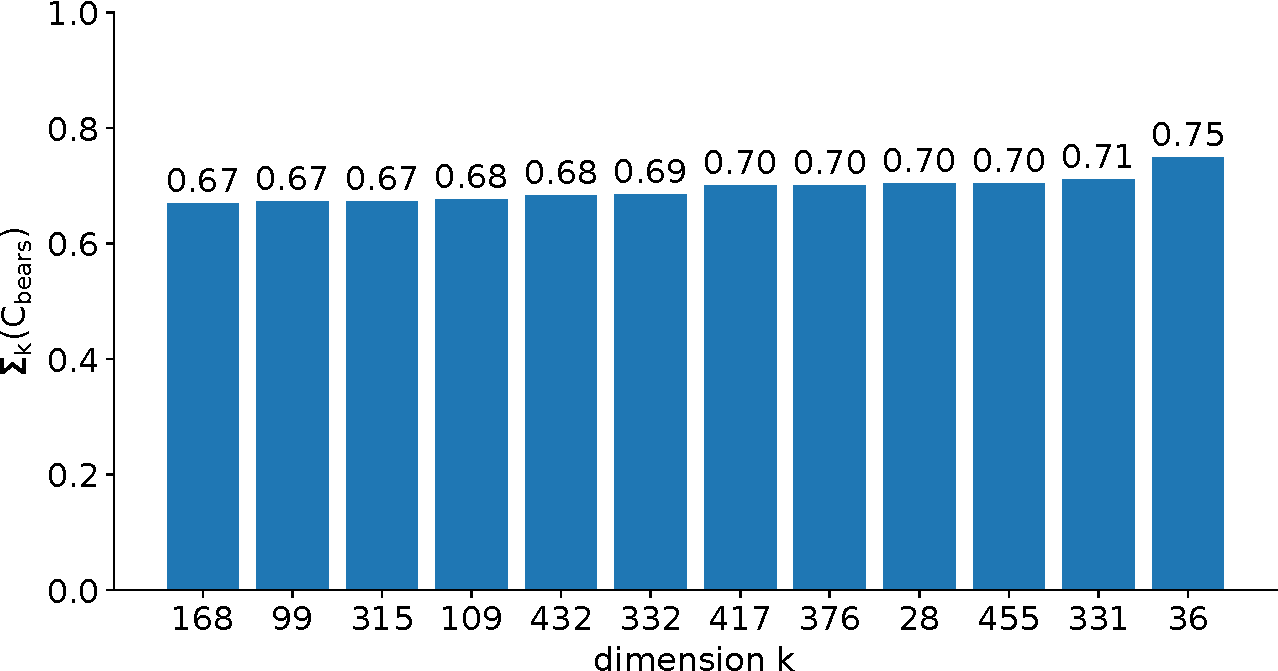
\includegraphics[width=\linewidth]{figures/highest_scores_barchart_ds19.pdf}
    \end{subfigure}
    \caption{A figure showing the 12 dimensions with the lowest $\Sigma$-scores (left) and the highest $\Sigma$-scores (right) in $C_{\text{bears}}$.}
    \label{fig:barcharts2}
\end{figure}

\begin{sidewaysfigure}
    \centering
    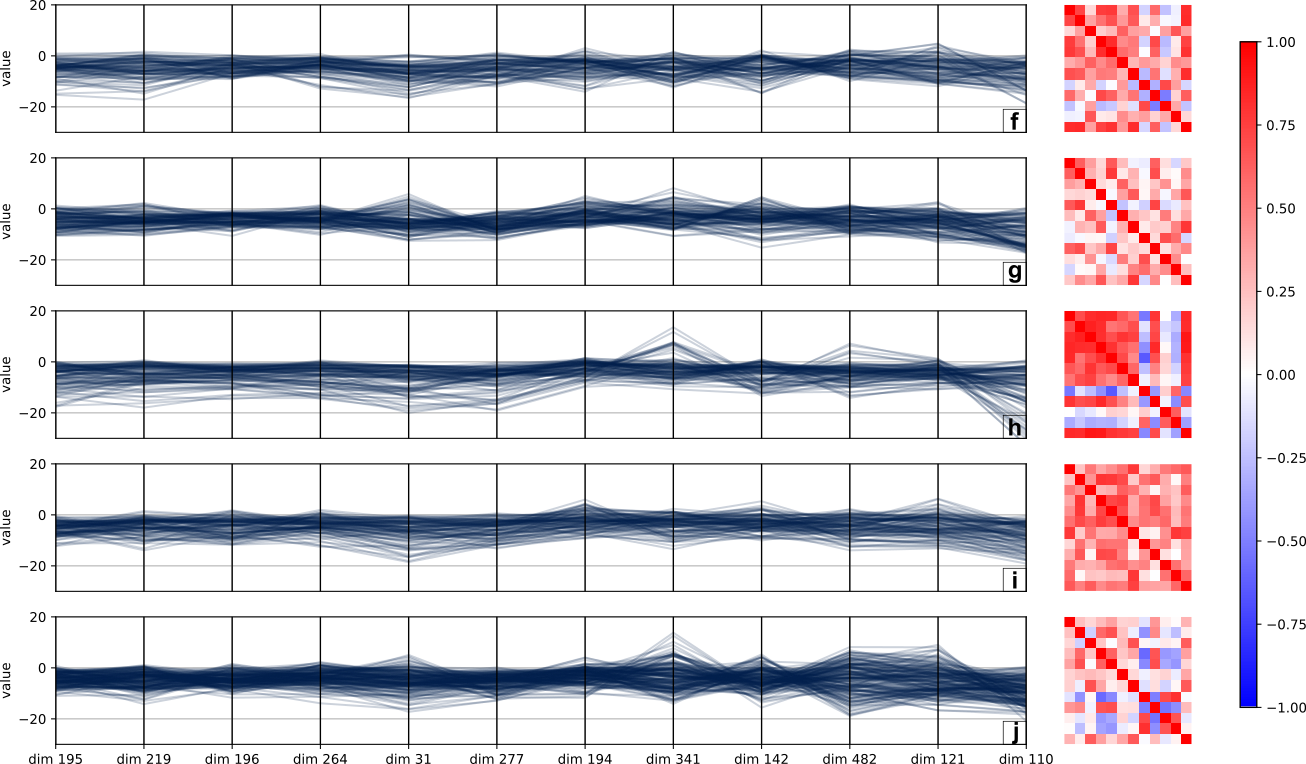
\includegraphics[width=\textheight]{figures/PCP_similar2.png}
    \caption{Five images of horses from BSD500 are segmented using the pipeline described in Chapter \ref{chapter:clustering_in_feature_space}. The feature vectors in the blue cluster of each segmentation result shown in \autoref{fig:classes} (f-j) are analyzed. The parallel coordinates plot shows the vectors of the corresponding cluster in the 12 dimensions with the highest $\Sigma$-scores (see \autoref{eq:E}). The correlation matrix of the dimensions (in their displayed order) is shown on the right.}
    \label{fig:pcp_similar2}
\end{sidewaysfigure}

\begin{sidewaysfigure}
    \centering
    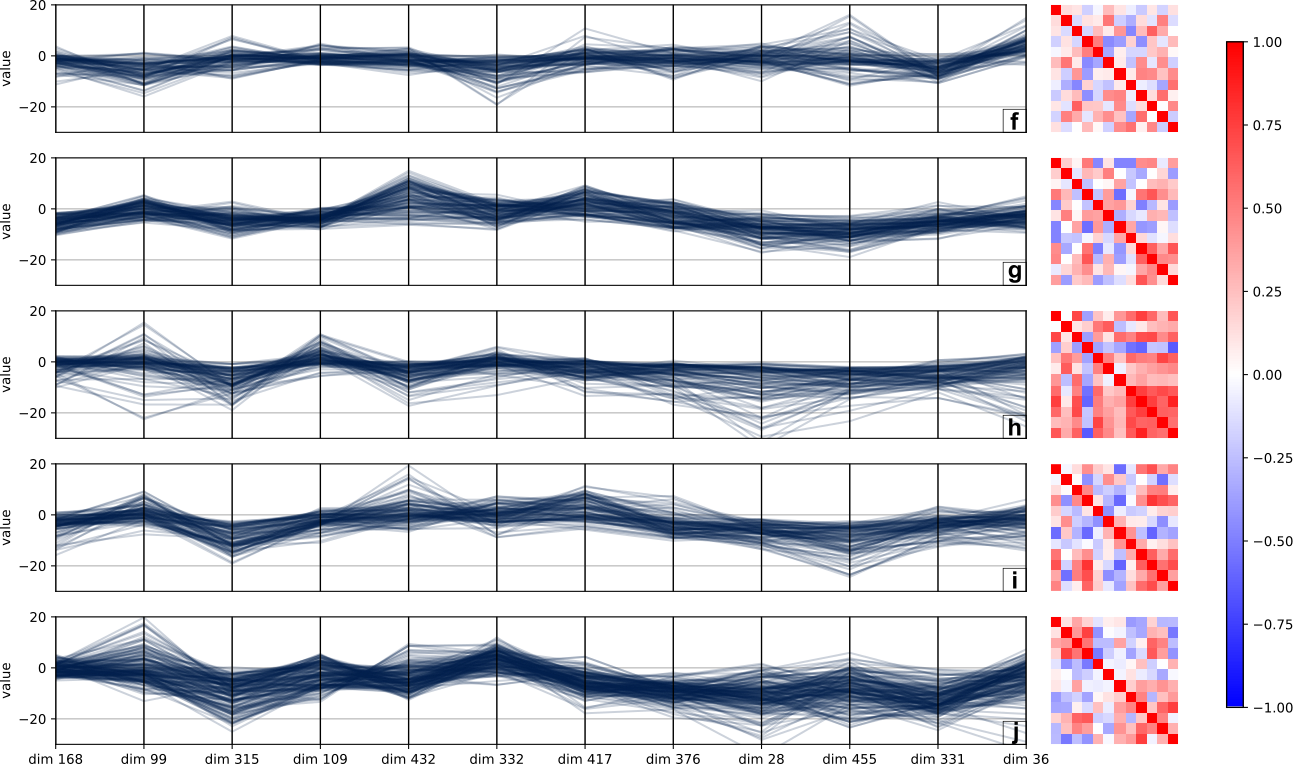
\includegraphics[width=\textheight]{figures/PCP_dissimilar2.png}
    \caption{Five images of horses from BSD500 are segmented using the pipeline described in Chapter \ref{chapter:clustering_in_feature_space}. The feature vectors in the blue cluster of each segmentation result shown in \autoref{fig:classes} (f-j) are analyzed. The parallel coordinates plot shows the vectors of the corresponding cluster in the 12 dimensions with the highest $\Sigma$-scores (see \autoref{eq:E}). The correlation matrix of the dimensions (in their displayed order) is shown on the right.}
    \label{fig:pcp_dissimilar2}
\end{sidewaysfigure}

\begin{figure}
    \centering
    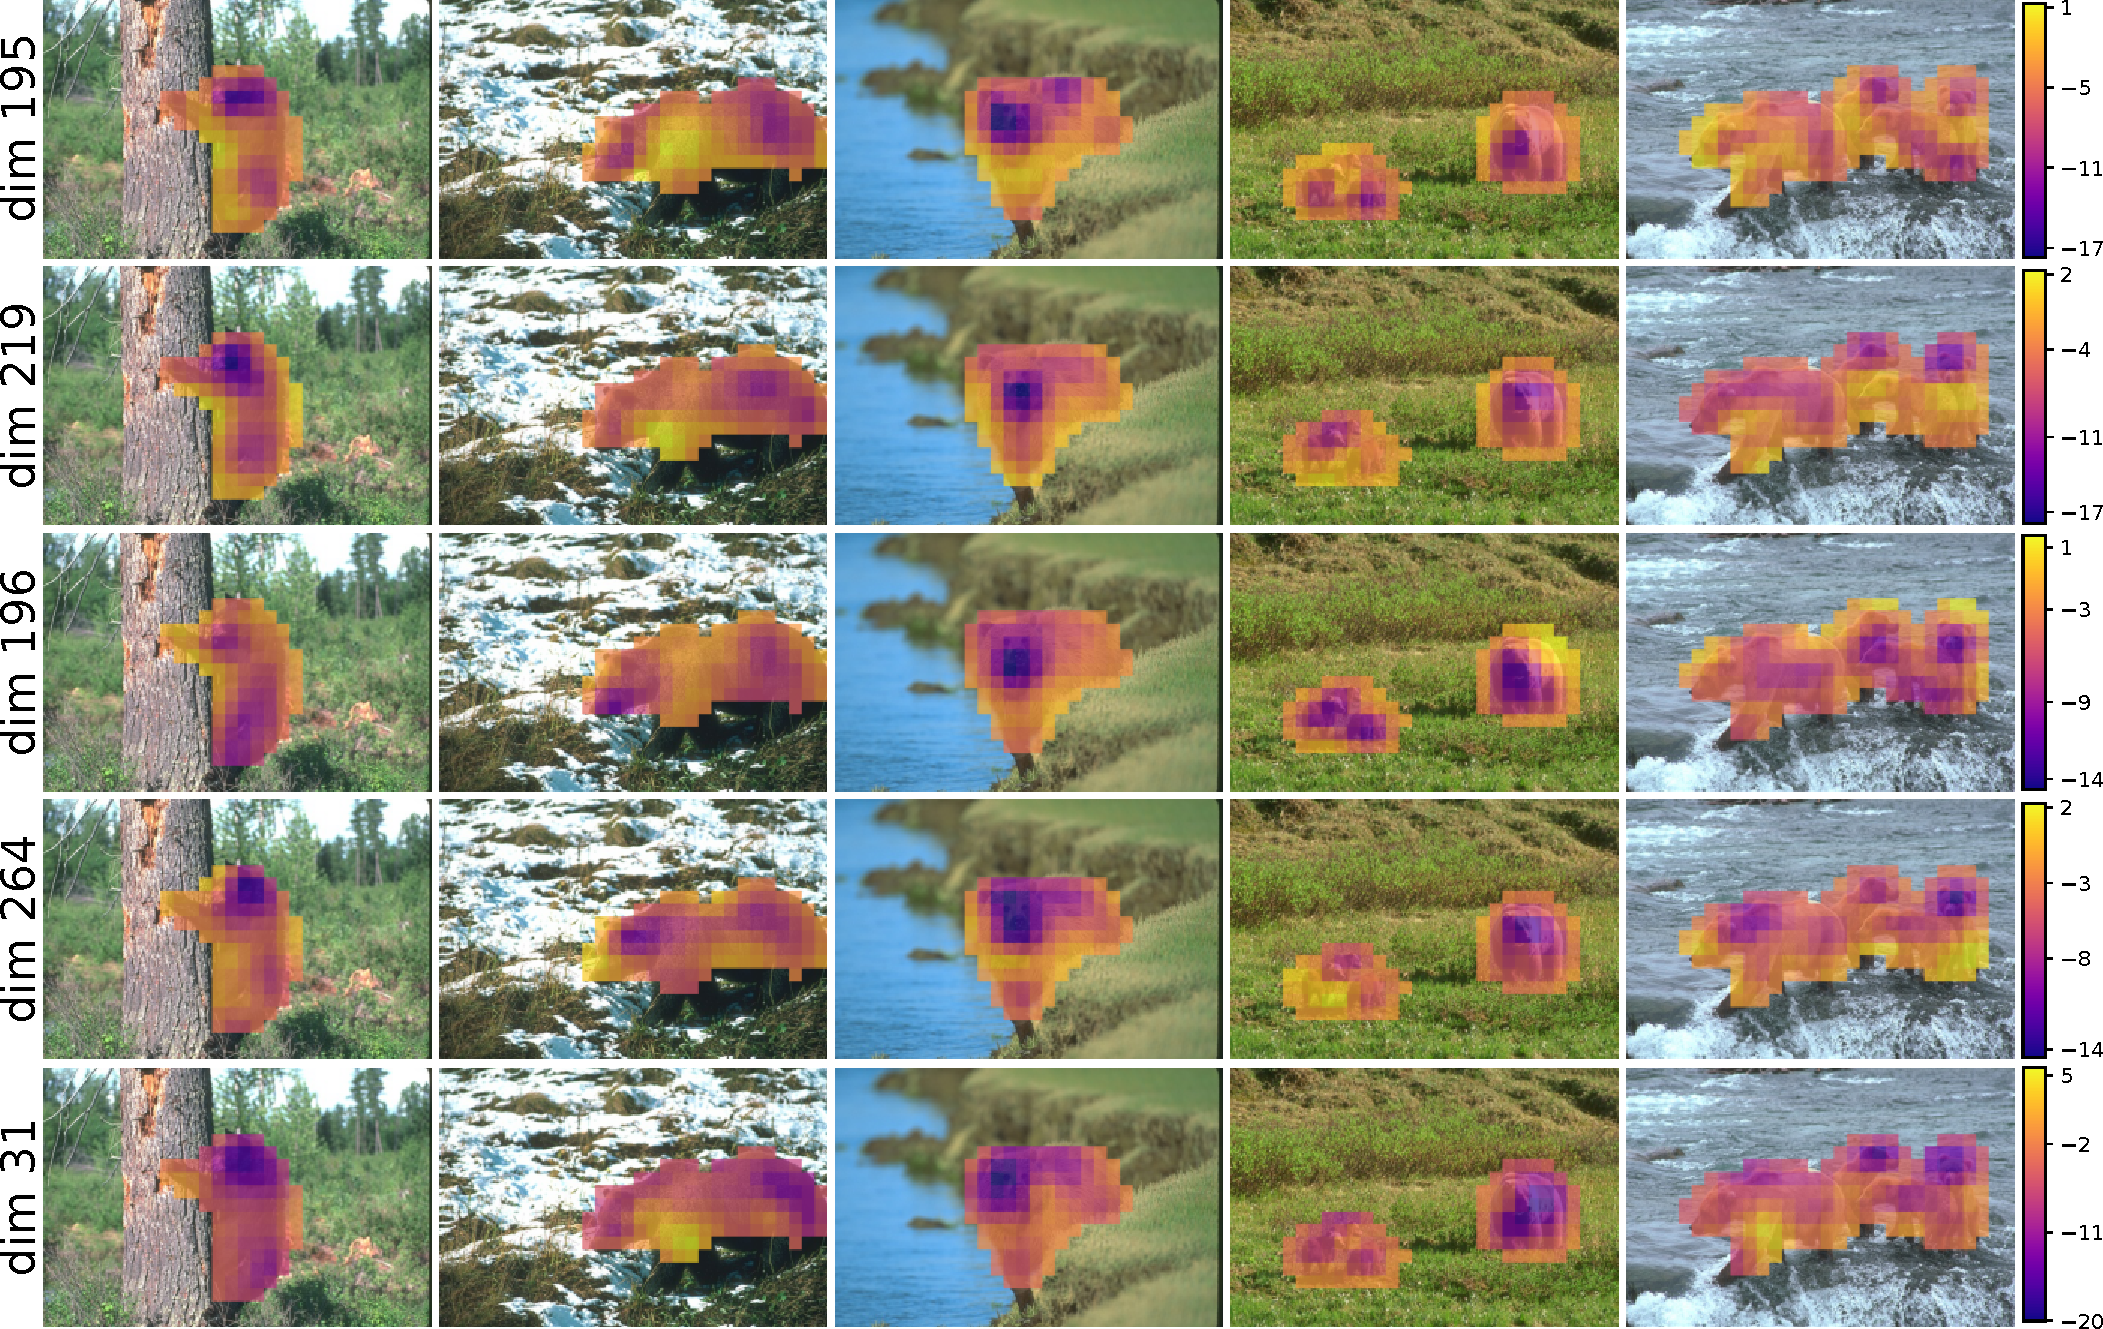
\includegraphics[width=.9\textwidth]{figures/overlayed_dim_similar2.pdf}
    \caption{The five lowest $\Sigma(C_{\text{bears}})$-scoring feature maps superimposed on their images.}
    \label{fig:overlay_similar_dims2}
\end{figure}

\begin{figure}
    \centering
    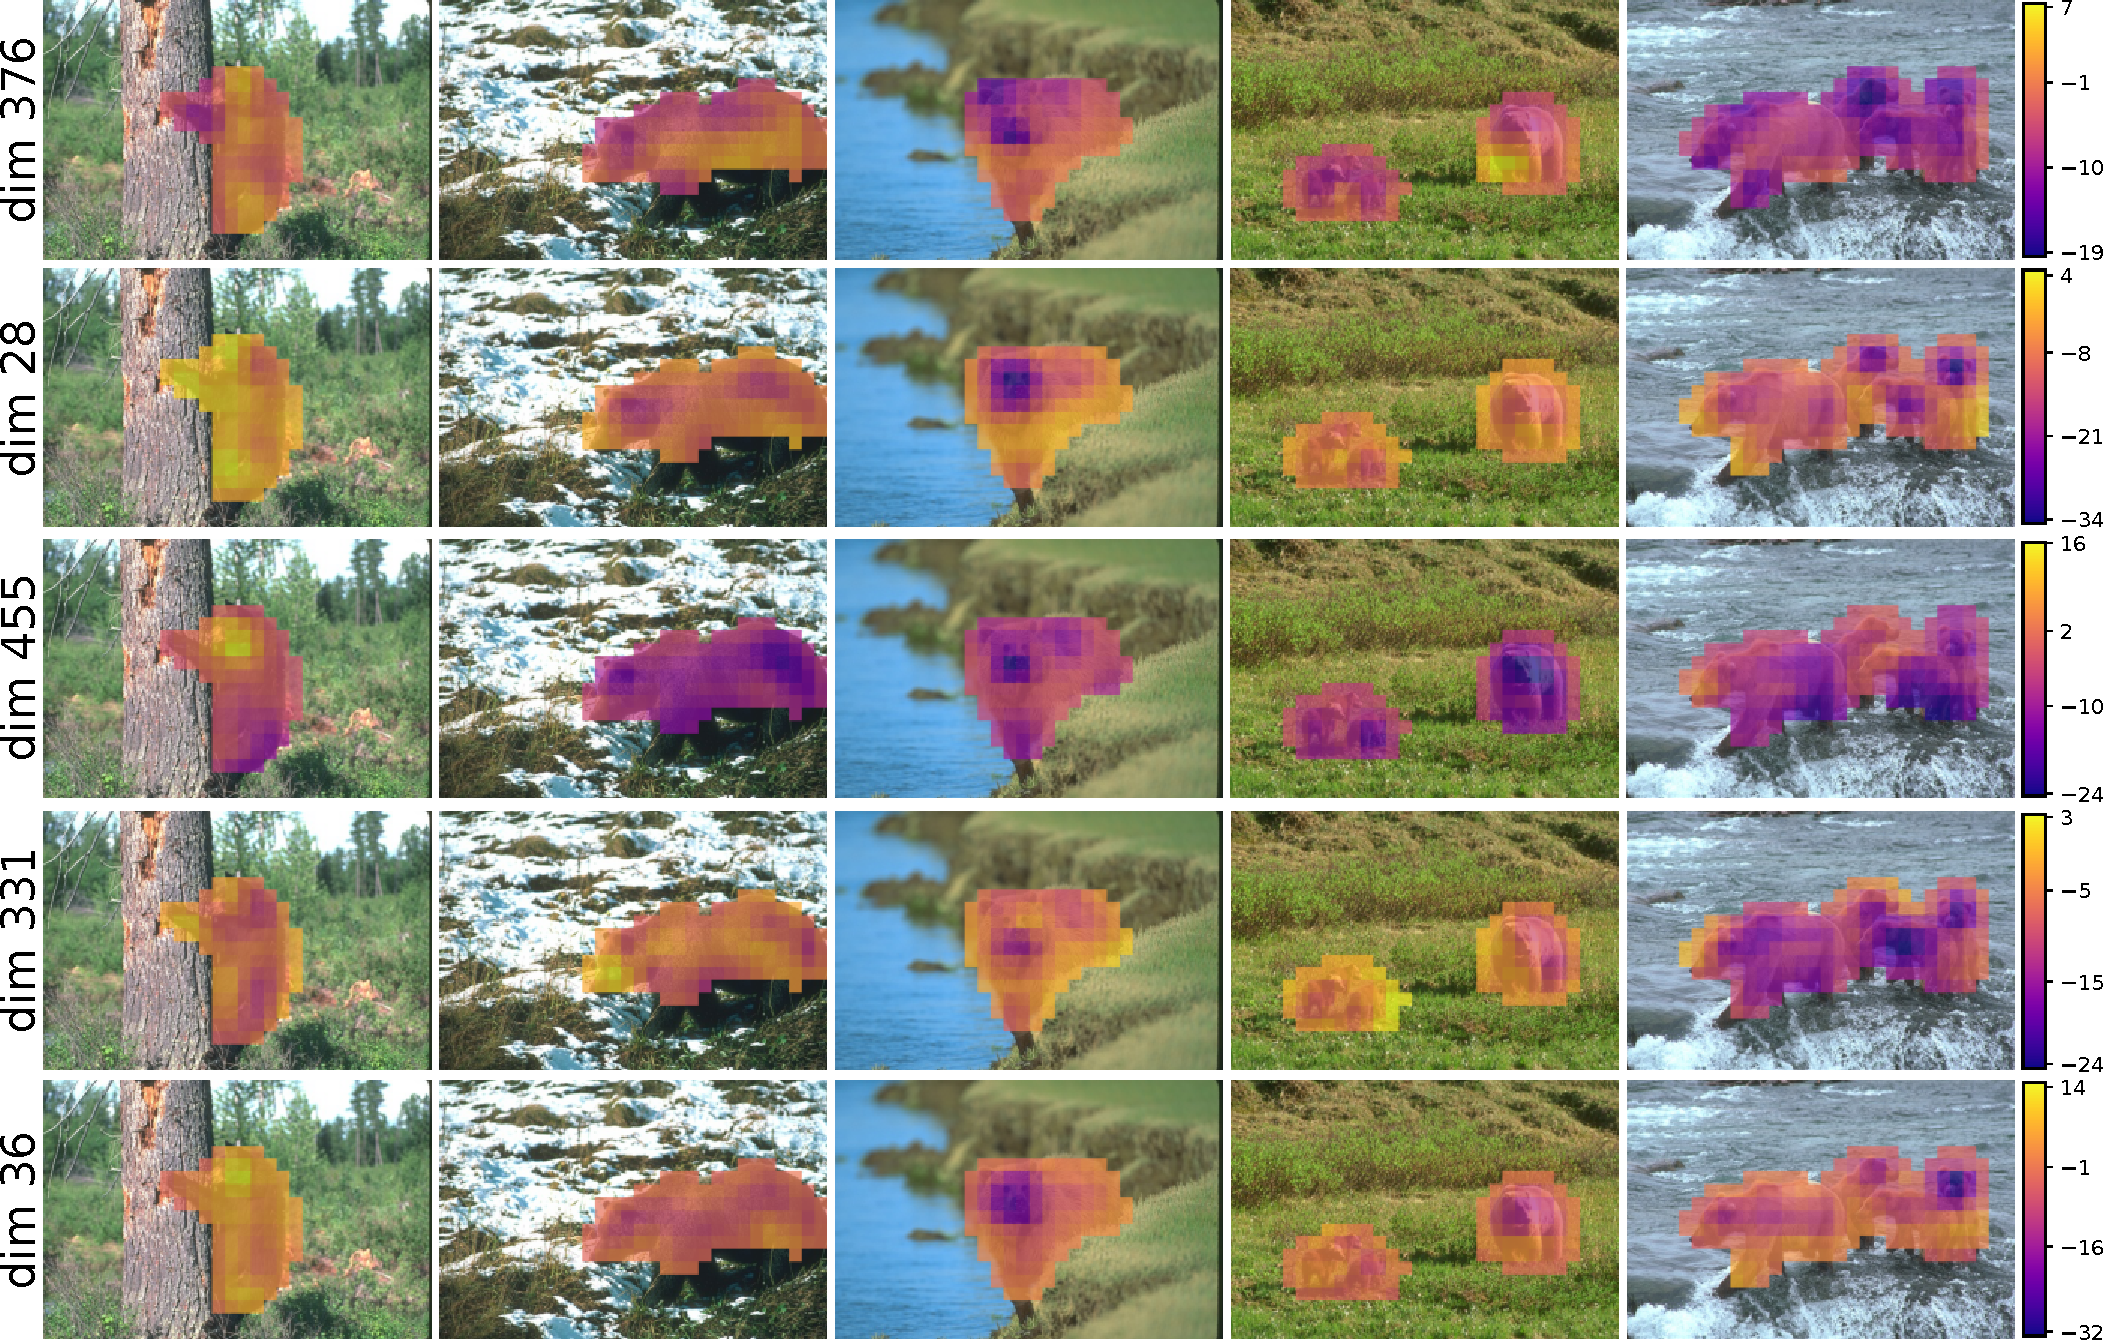
\includegraphics[width=.9\textwidth]{figures/overlayed_dim_dissimilar2.pdf}
    \caption{The five highest $\Sigma(C_{\text{bears}})$-scoring feature maps superimposed on their images.}
    \label{fig:overlay_dissimilar_dims2}
\end{figure}

\section{Empirical Cumulative Distribution Functions}

In \autoref{section:further_analysis}, two classes containing five semantically similar images from BSD500 were segmented (see \autoref{fig:classes}).
The feature maps of the objects in the foreground were analyzed to discover their similarities and differences. The ECDFs of the 12 lowest- and highest-$\Sigma$-scoring feature maps are shown in \autoref{fig:ecdfs} for $C_{\text{horses}}$ and in \autoref{fig:ecdfs2} for $C_{\text{bears}}$.

\begin{figure}[t]
    \centering
    \begin{subfigure}{\textwidth}
        \centering
        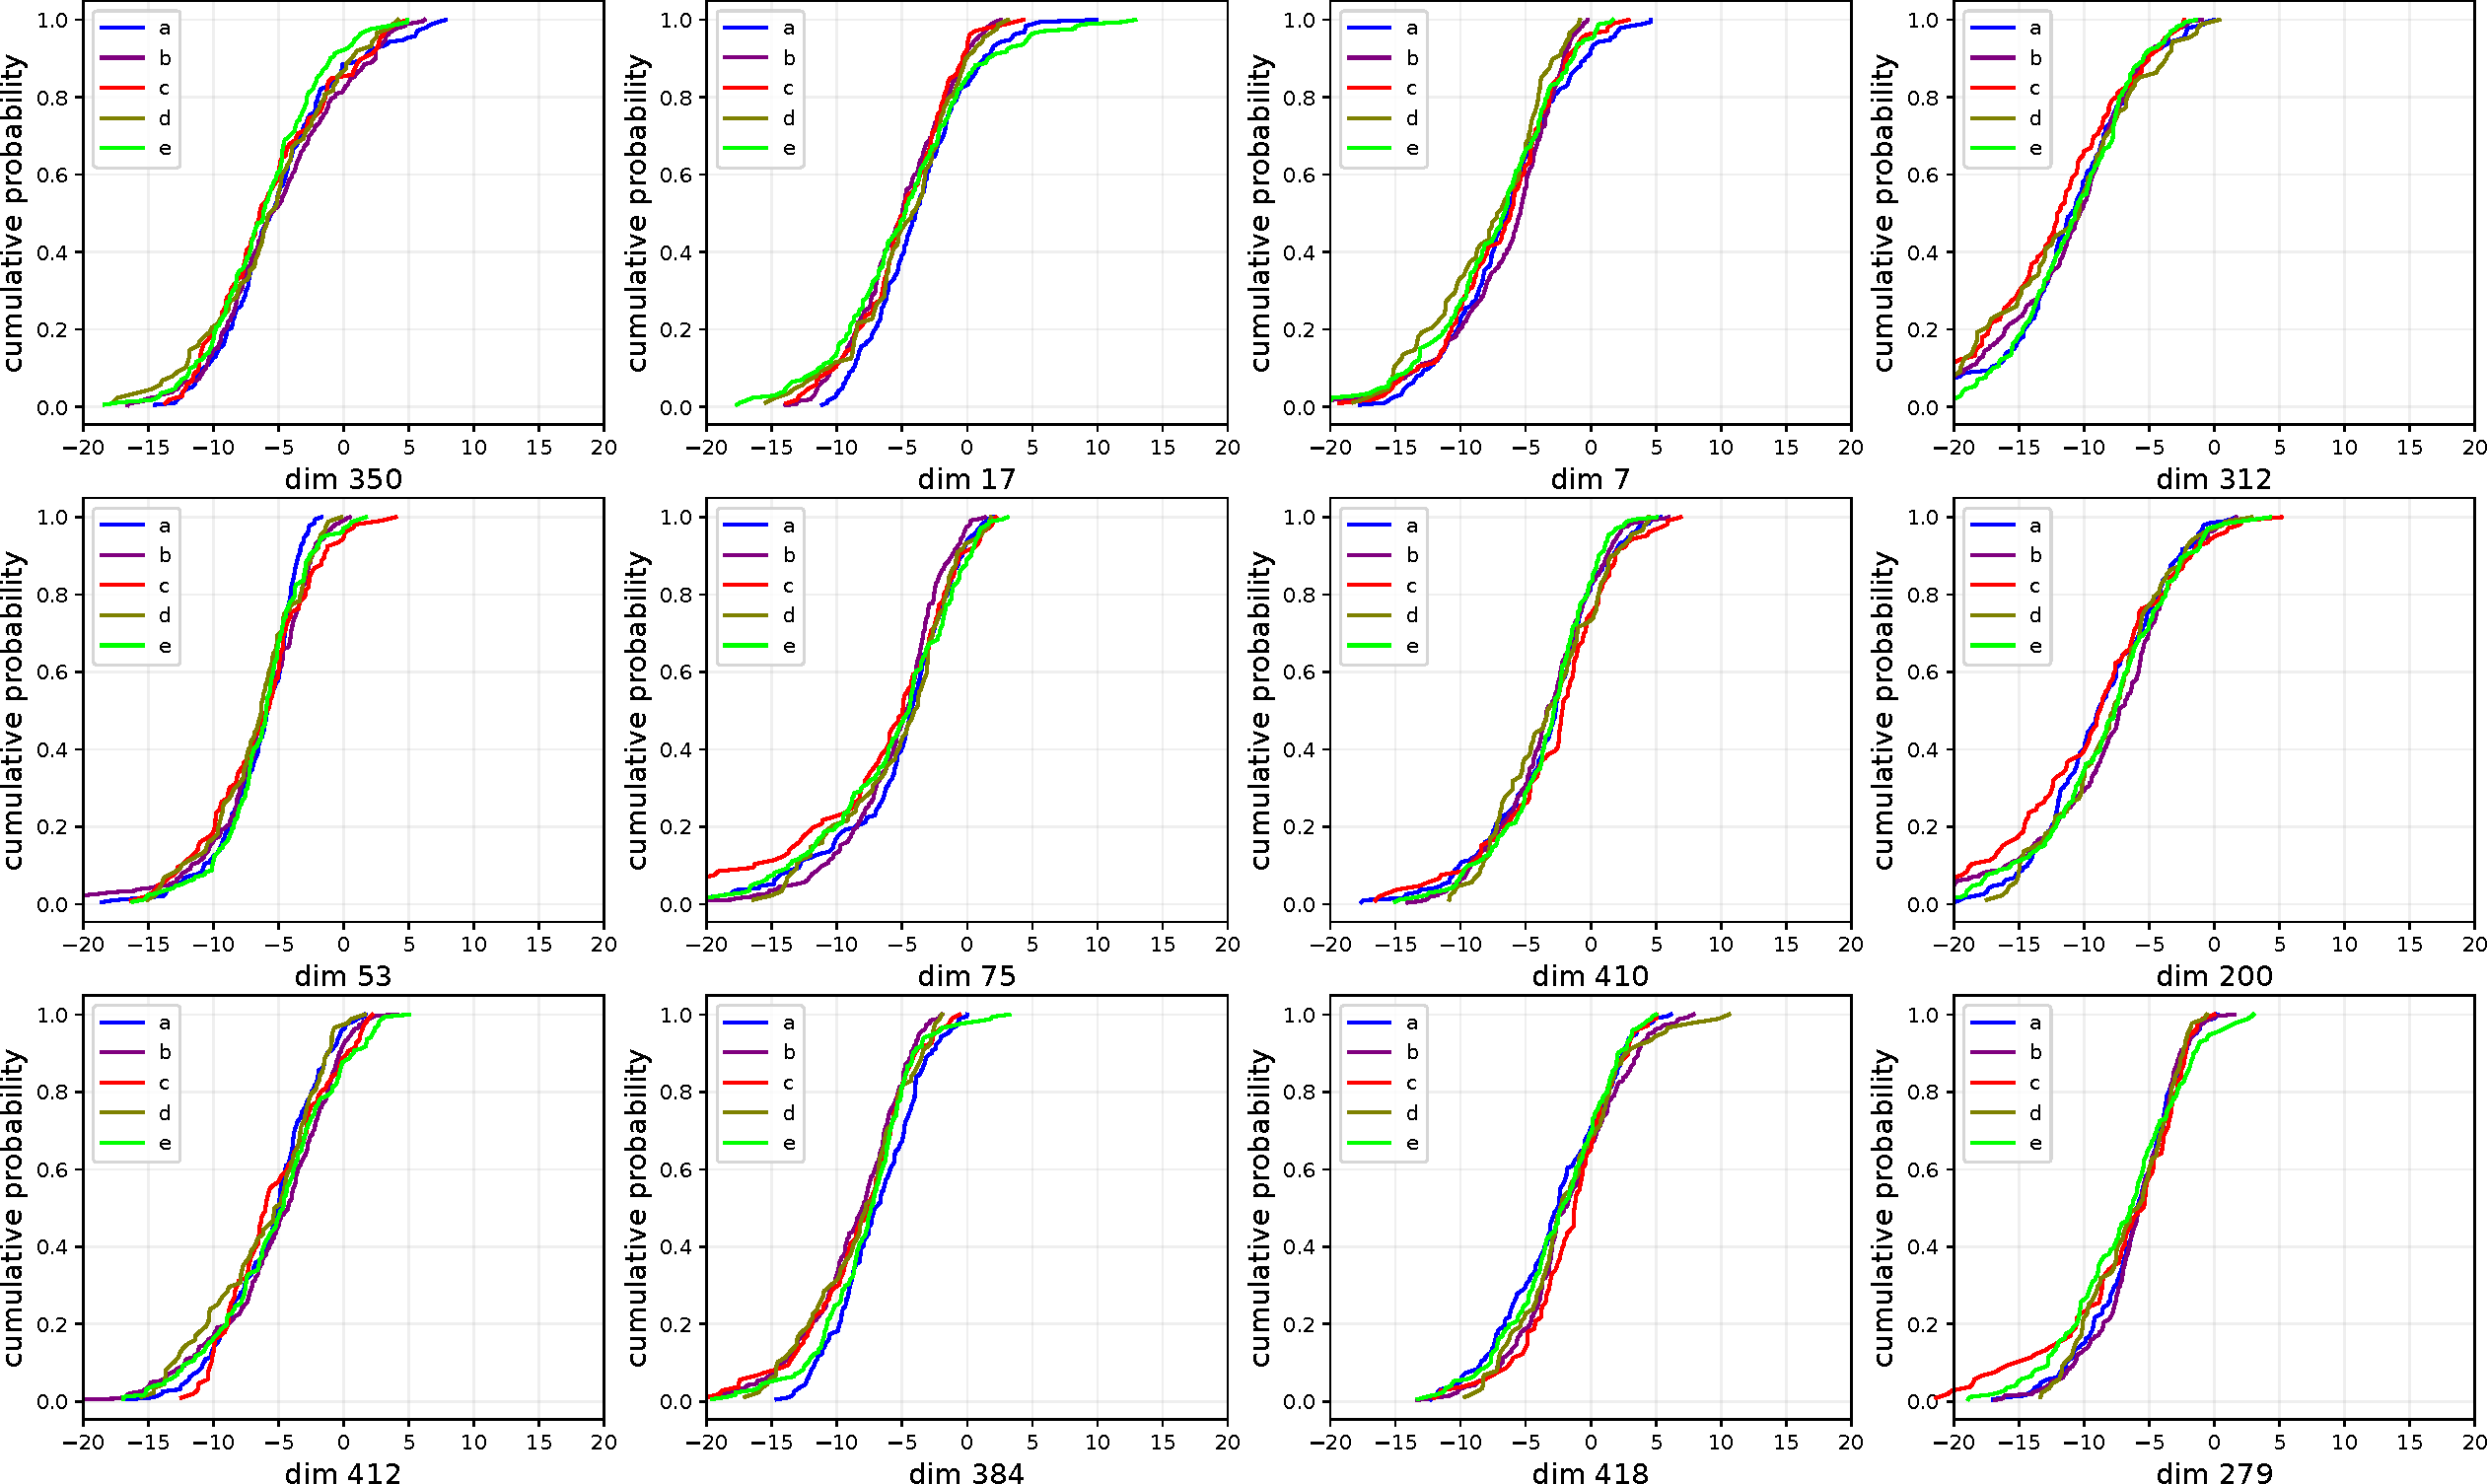
\includegraphics[width=.85\linewidth]{figures/ECDFs_similar.pdf}
    \vspace{5mm}
    \end{subfigure}
    \begin{subfigure}{\textwidth}
        \centering
        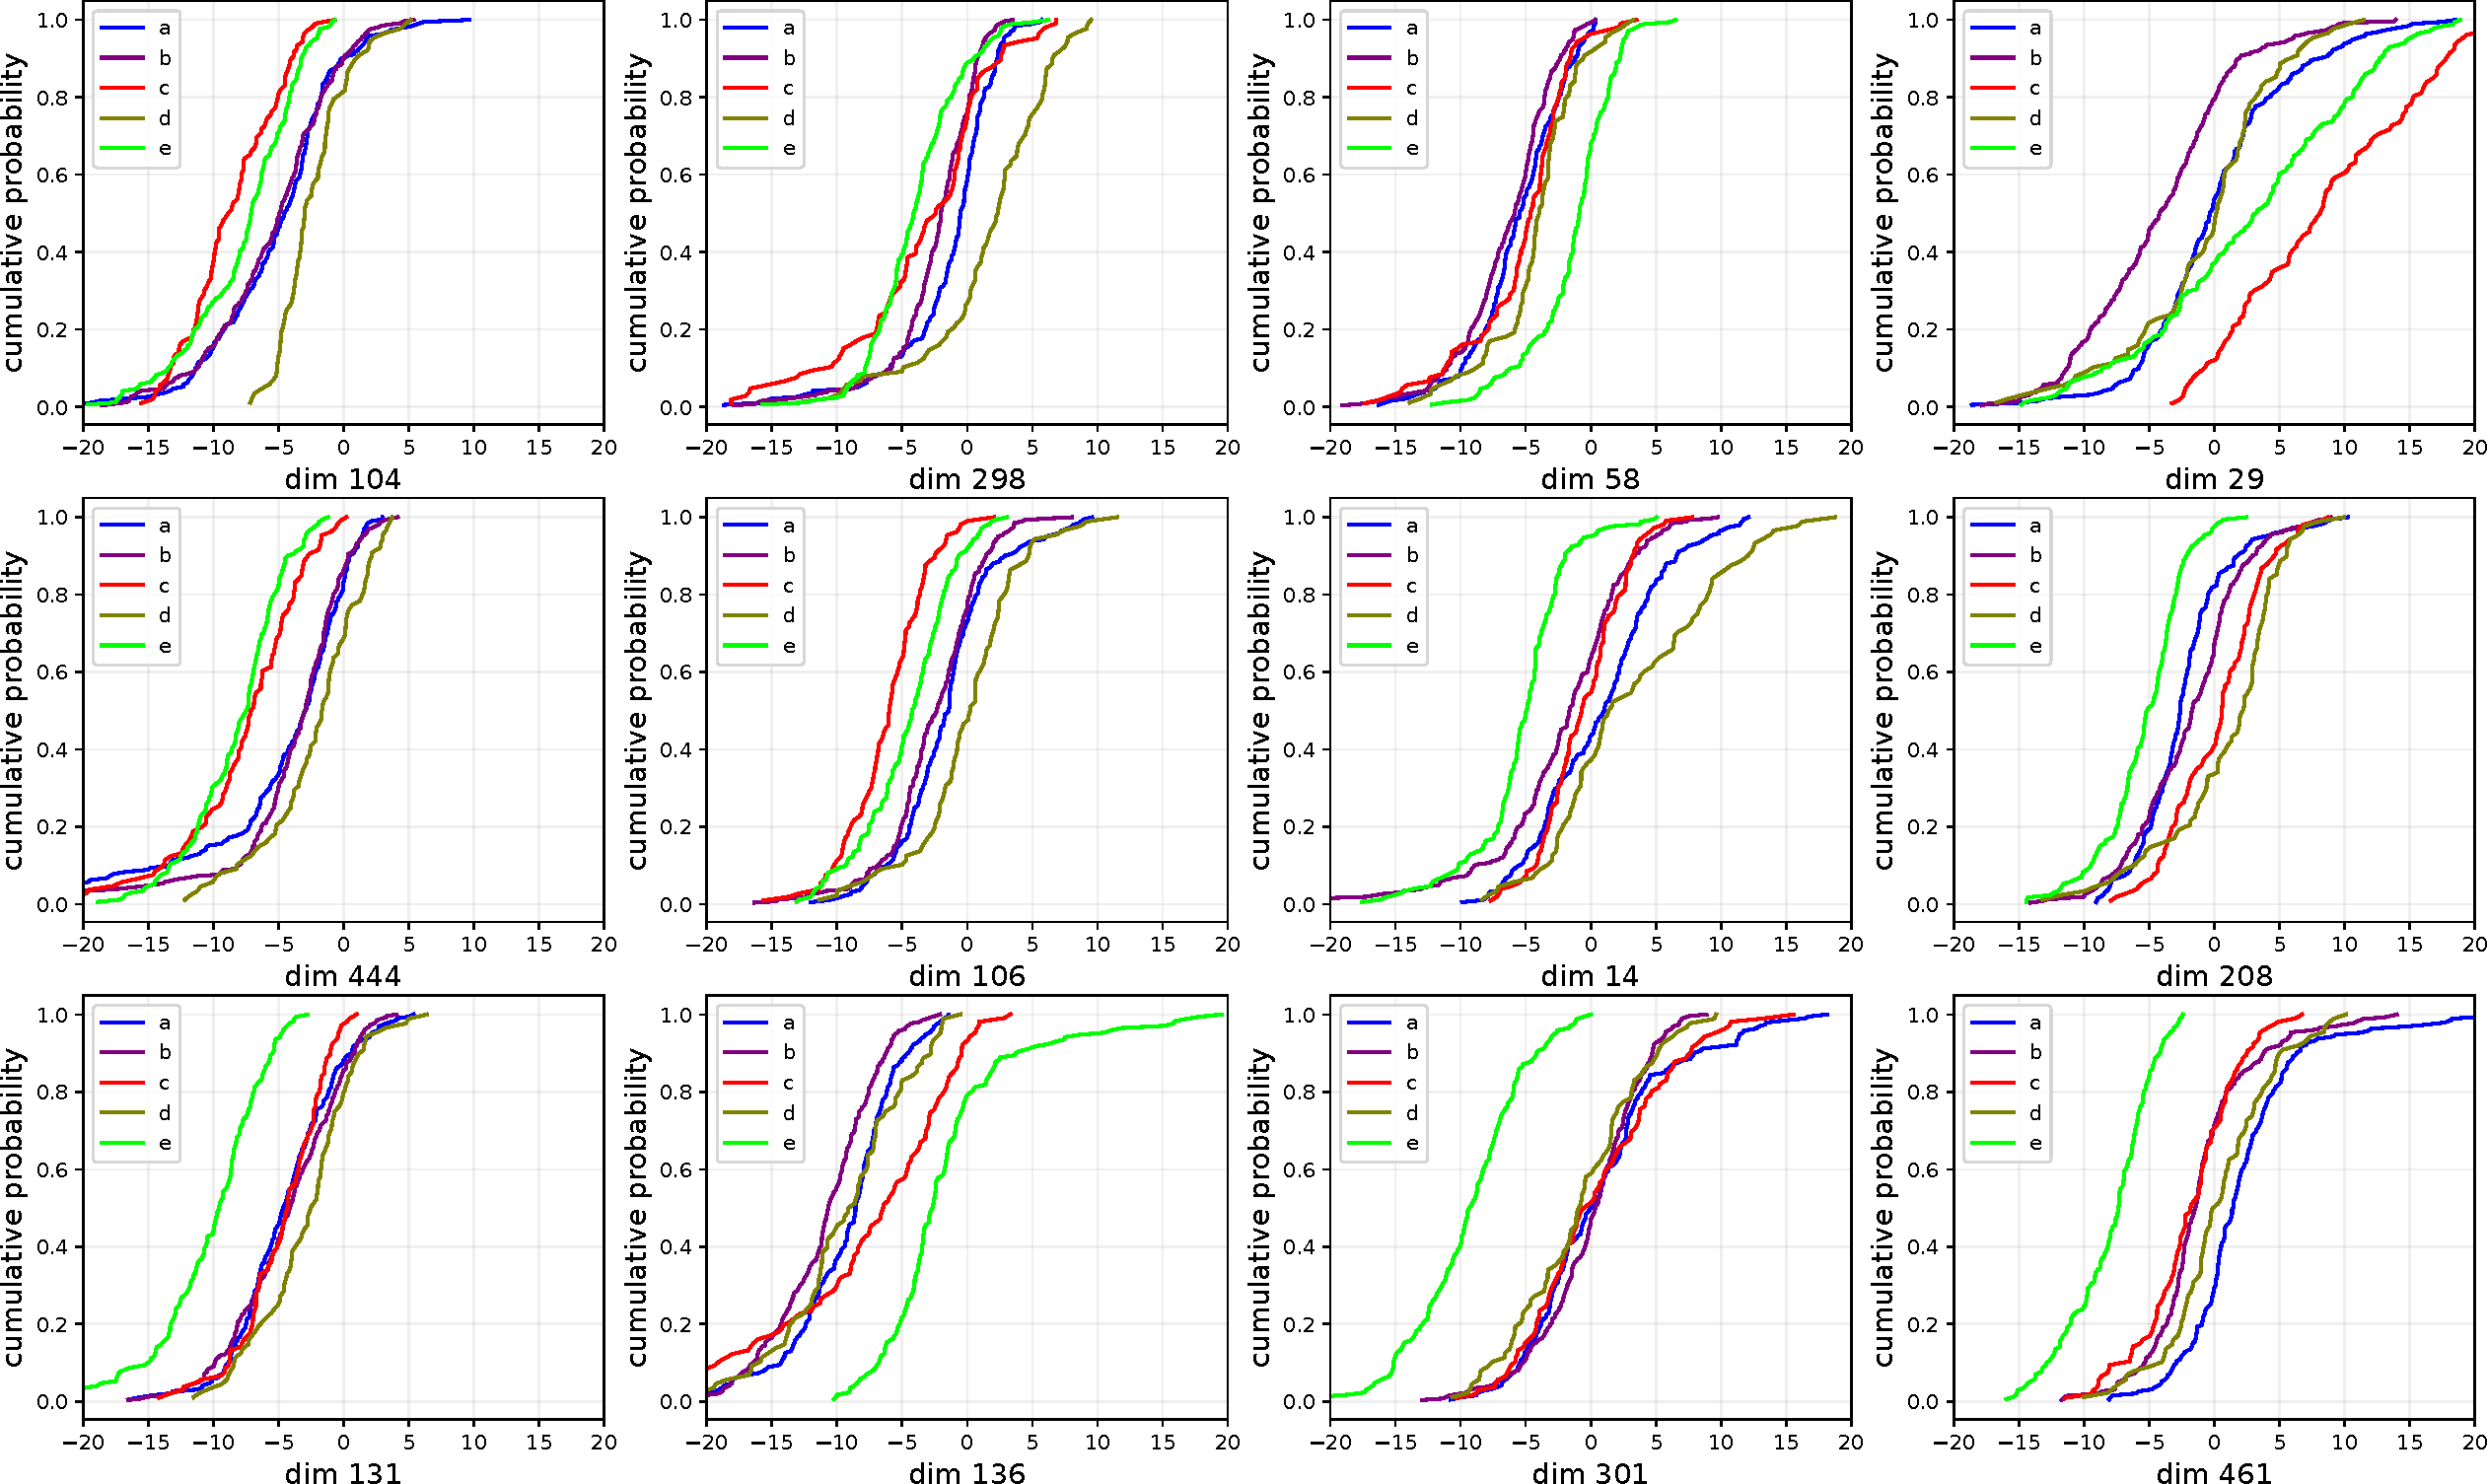
\includegraphics[width=.85\linewidth]{figures/ECDFs_dissimilar.pdf}
    \end{subfigure}
    \caption{The ECDFs of the dimensions shown in \autoref{fig:barcharts}.}
    \label{fig:ecdfs}
\end{figure}

\begin{figure}[t]
    \centering
    \begin{subfigure}{\textwidth}
        \centering
        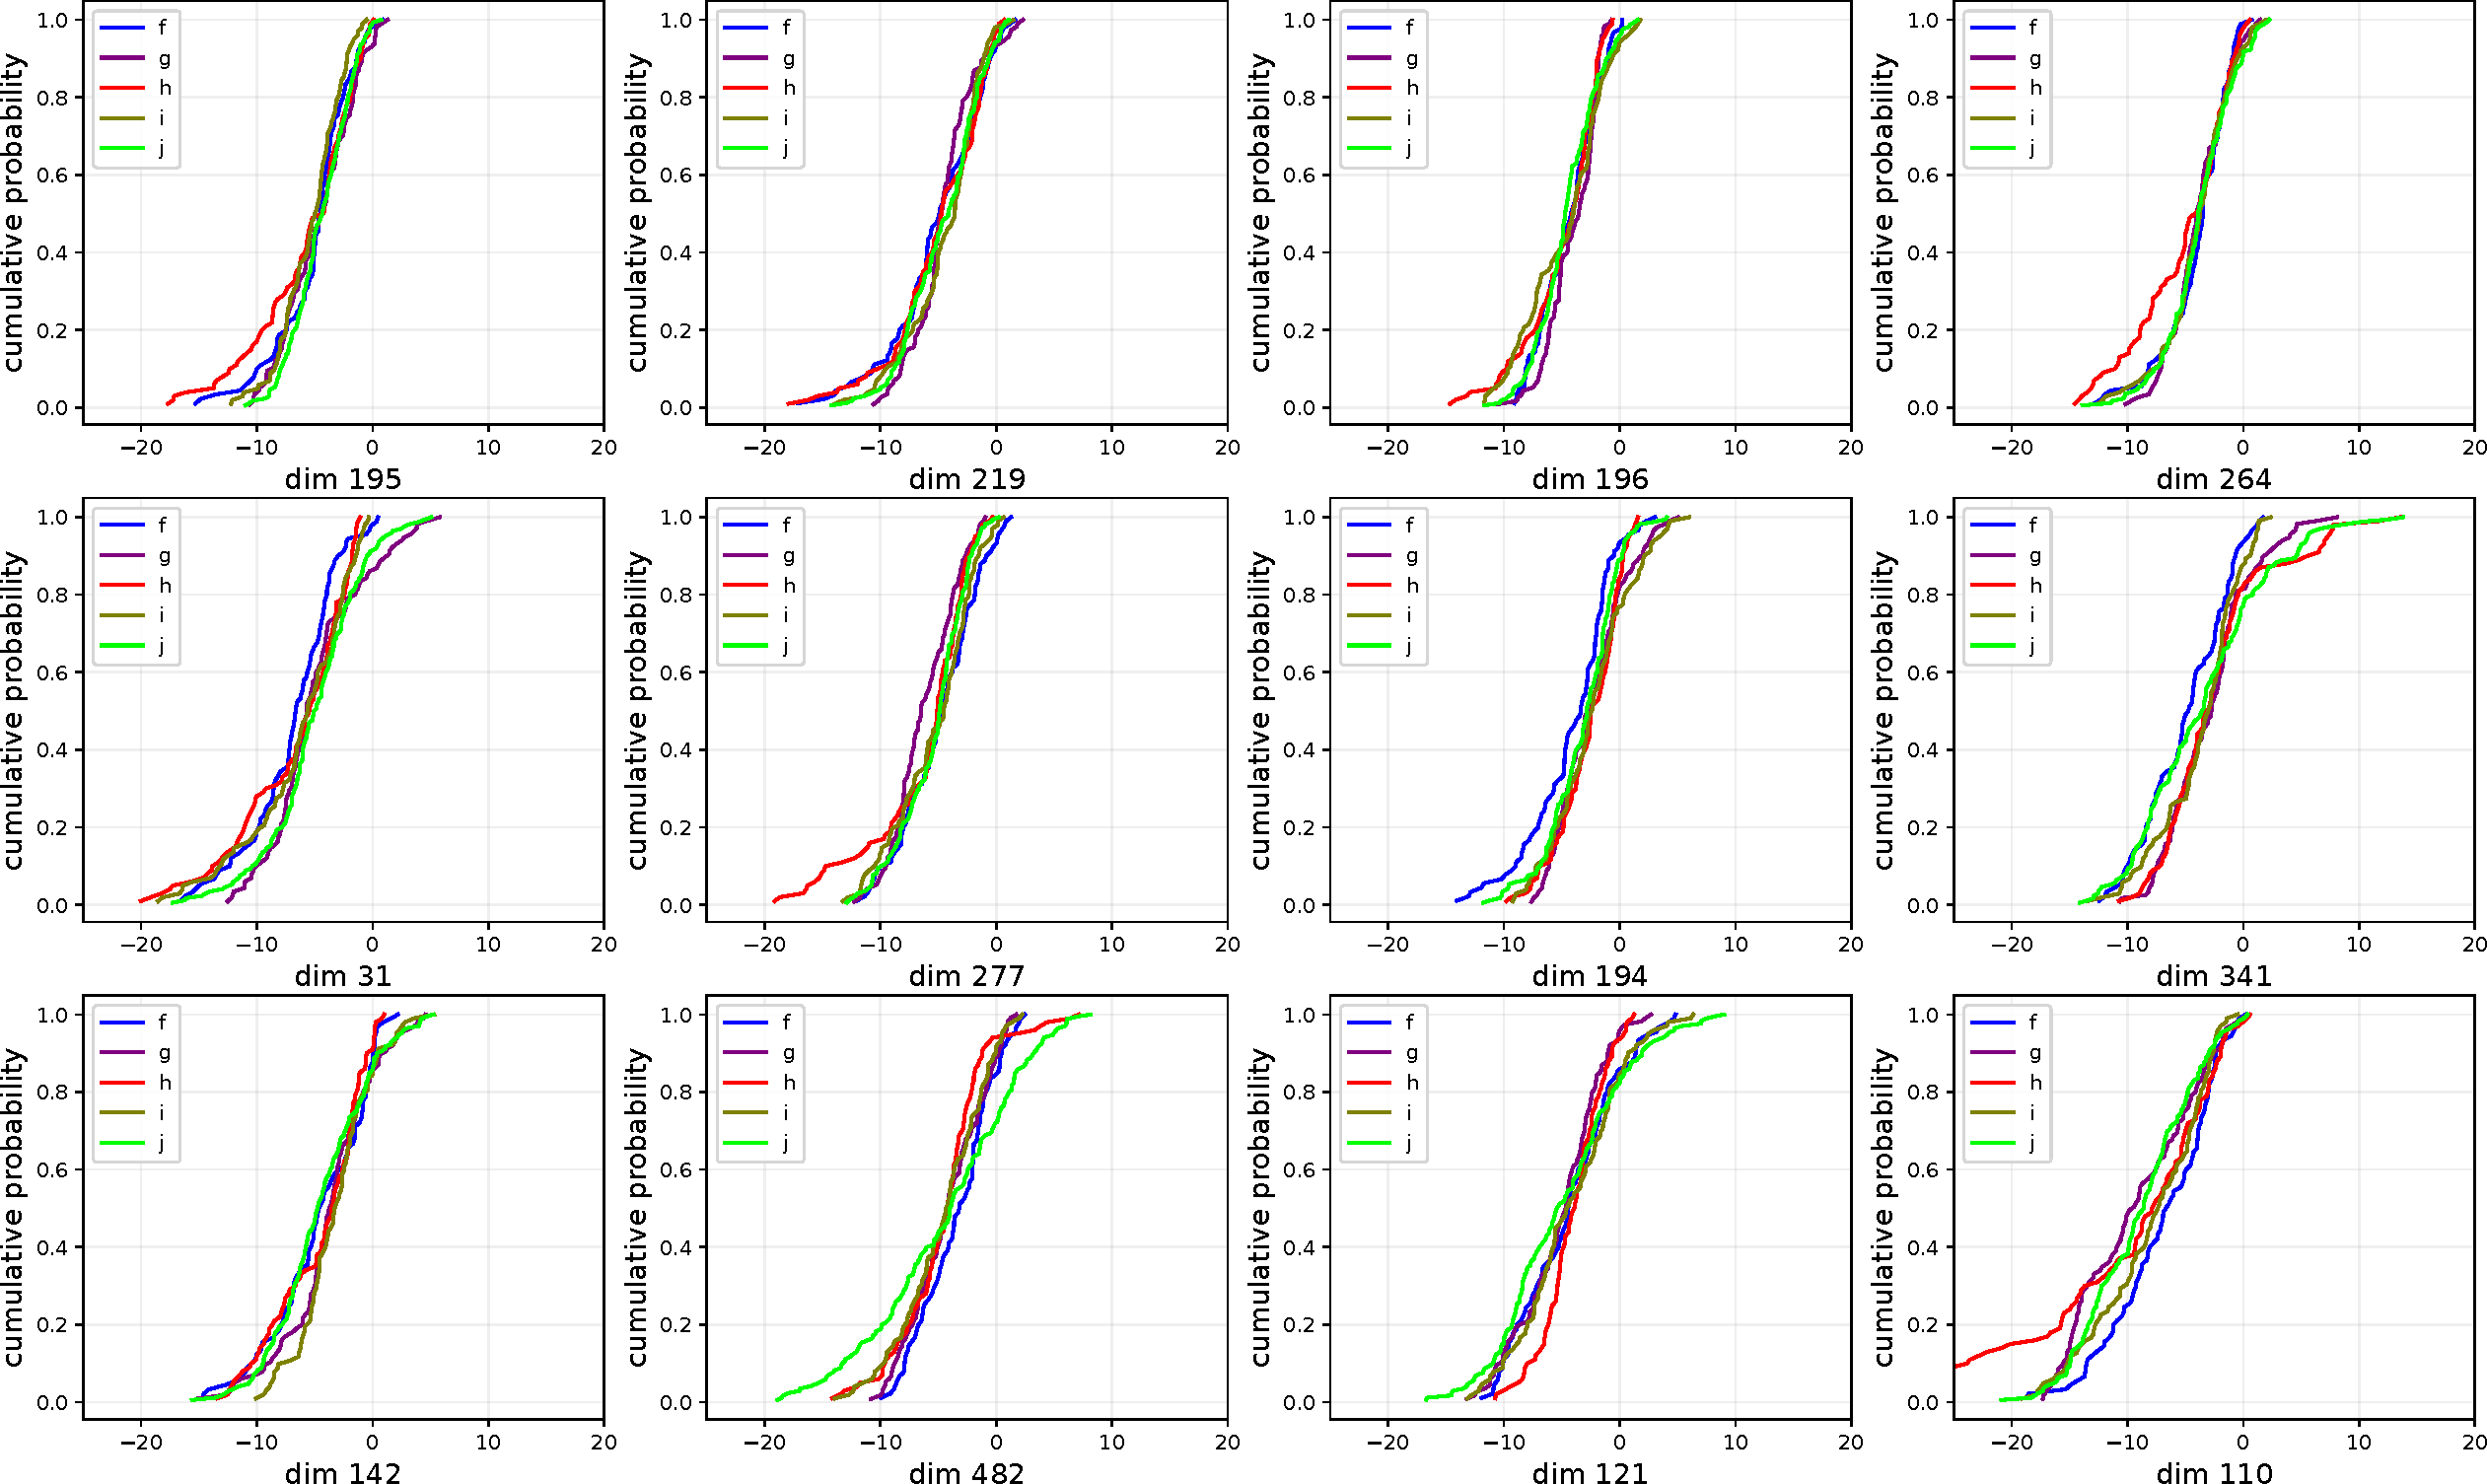
\includegraphics[width=.85\linewidth]{figures/ECDFs_similar2.pdf}
    \vspace{5mm}
    \end{subfigure}
    \begin{subfigure}{\textwidth}
        \centering
        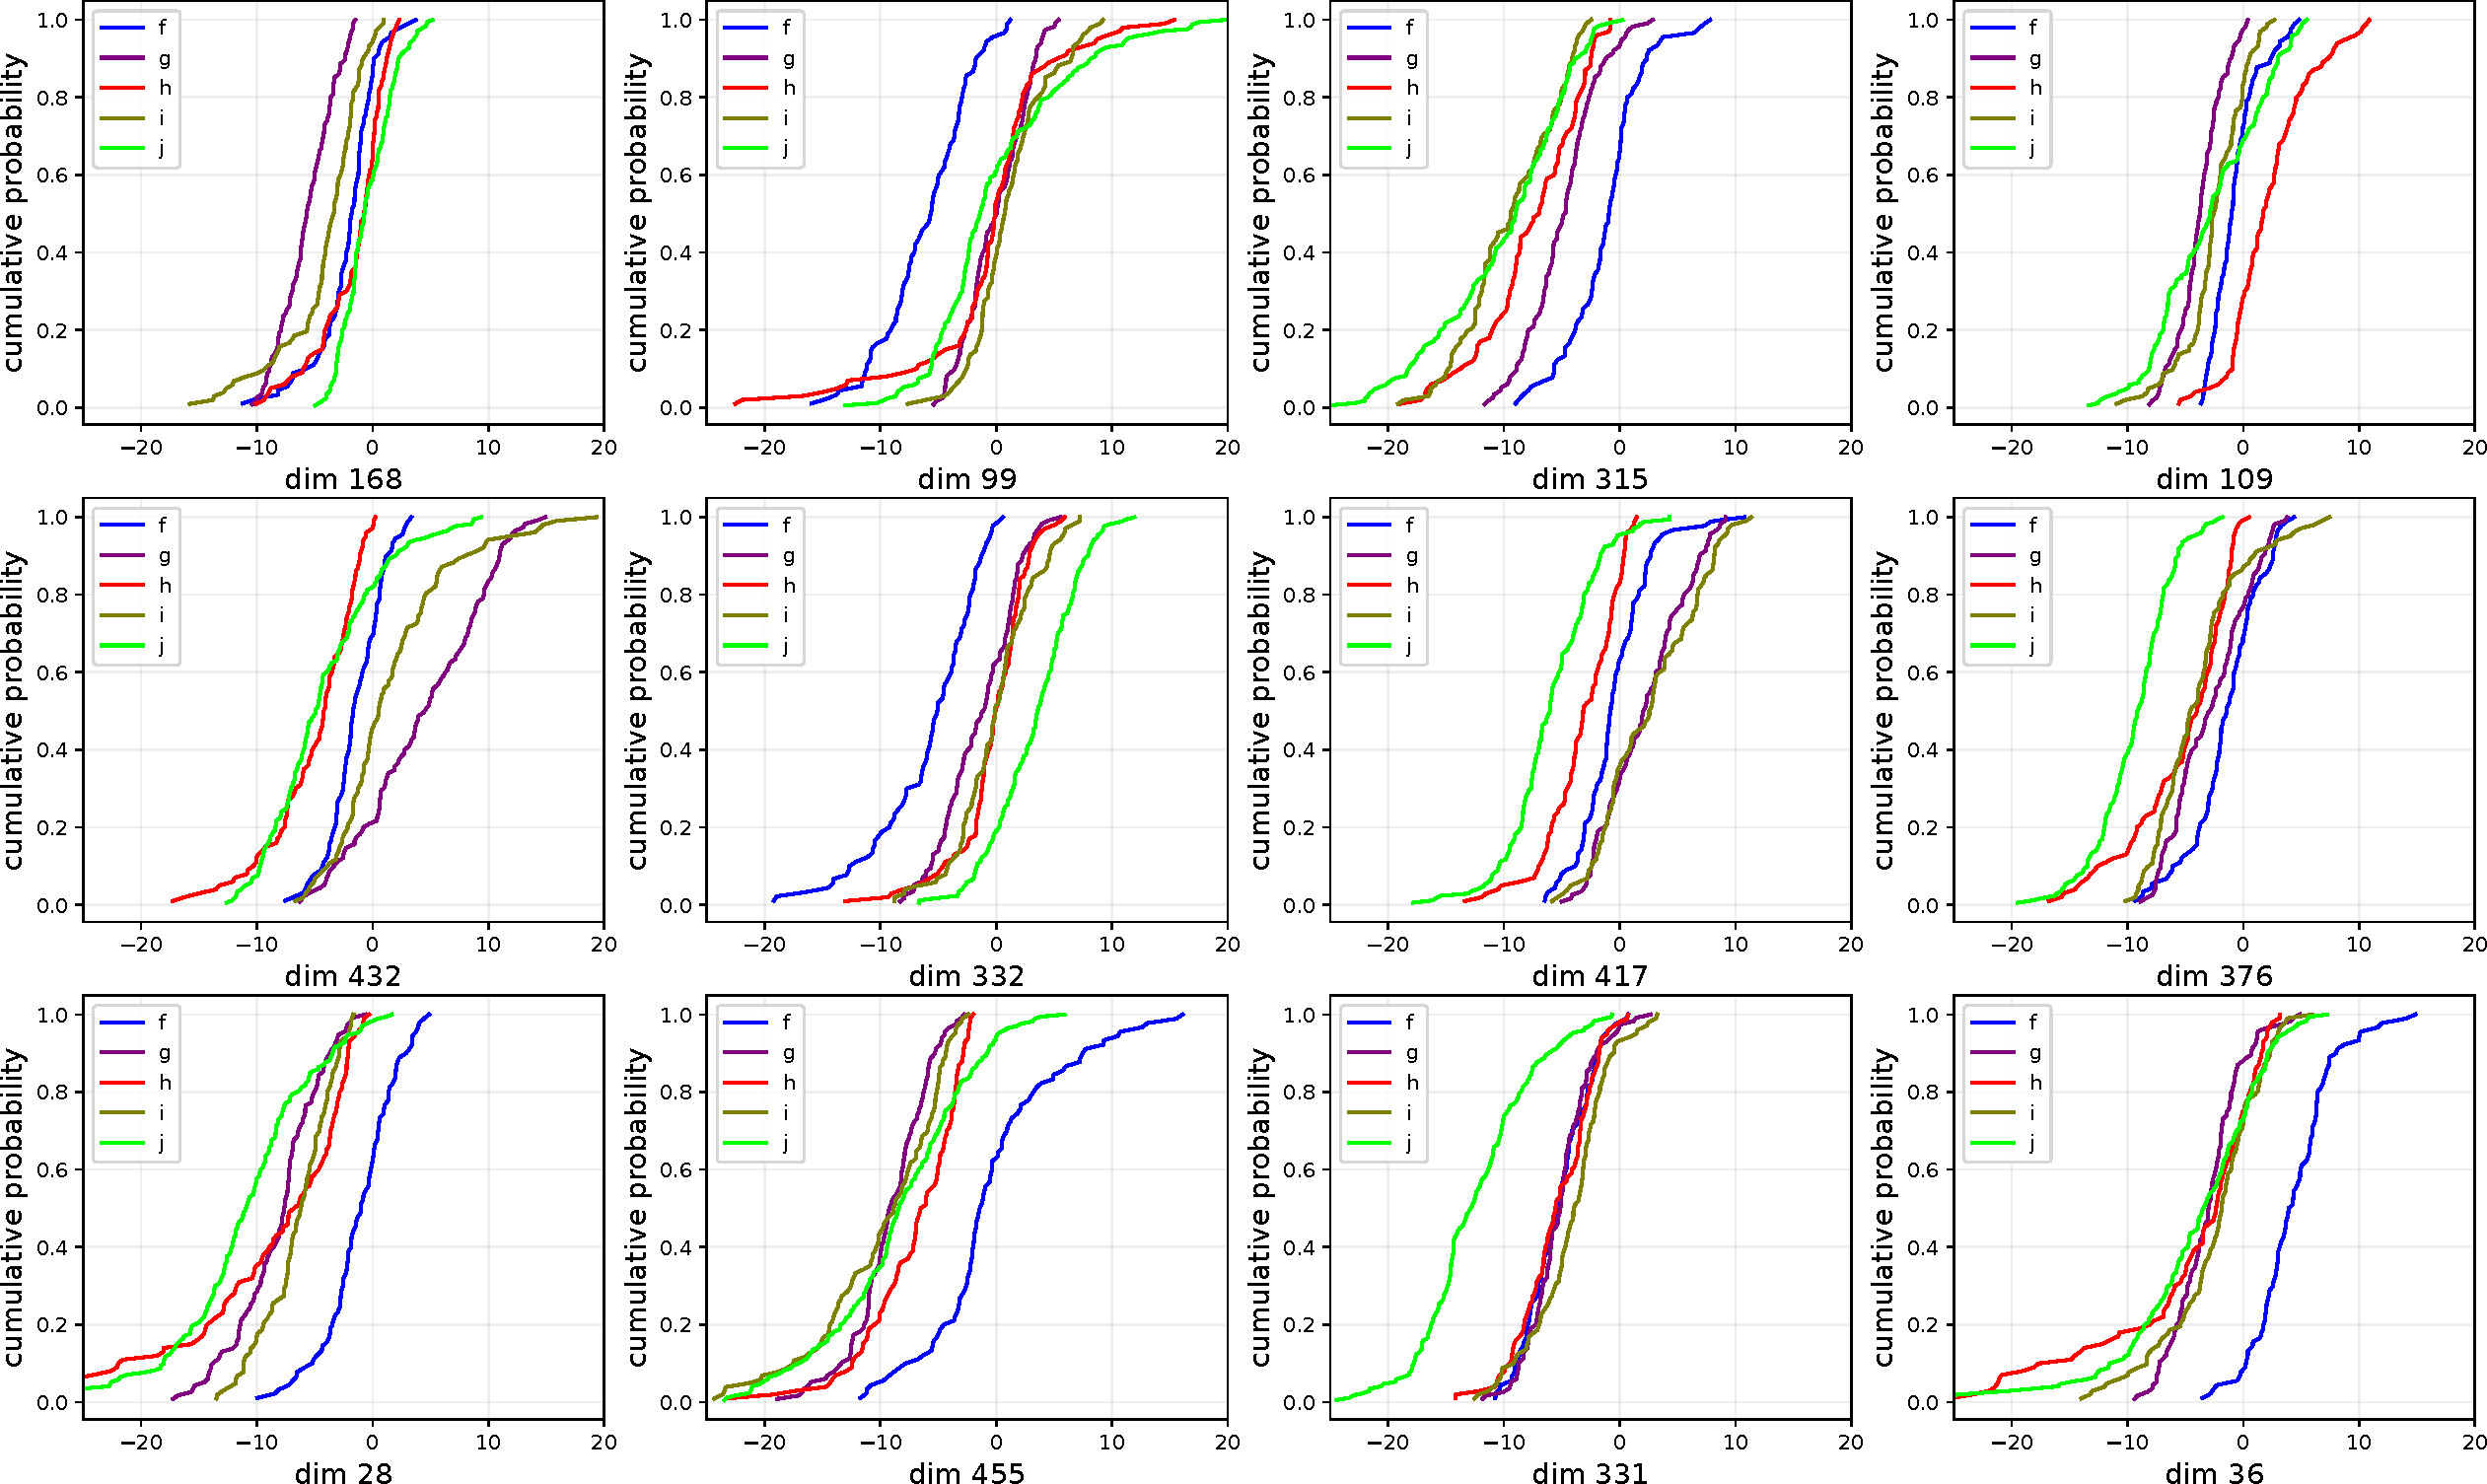
\includegraphics[width=.85\linewidth]{figures/ECDFs_dissimilar2.pdf}
    \end{subfigure}
    \caption{The ECDFs of the dimensions shown in \autoref{fig:barcharts2}.}
    \label{fig:ecdfs2}
\end{figure}

\clearpage
\chapter{Contour Refinement}\label{chapter:contour_refinement}

The segmentation pipeline discussed in \autoref{chapter:clustering_in_feature_space} generated a segmentation mask by grouping pixels in the feature image. One disadvantage of using the feature image is that it has a lower spatial resolution than the original image. This is due to the downsampling introduced by the max pooling layers in the VGG16. As a result, accurate boundary information between two adjacent regions is lost. The lower resolution segmentation mask does not have enough pixels to represent the different contours accurately. In order to address this issue, some of the methods proposed in the literature can be reused for refining the final segmentation mask \parencite{ma2018fully}. In this section, we investigate restoring some of the original contours of the segmentation image by using the superpixel color image. \autoref{fig:smv} outlines the process described in this subsection.

\begin{figure}[htbp]
    \centering
    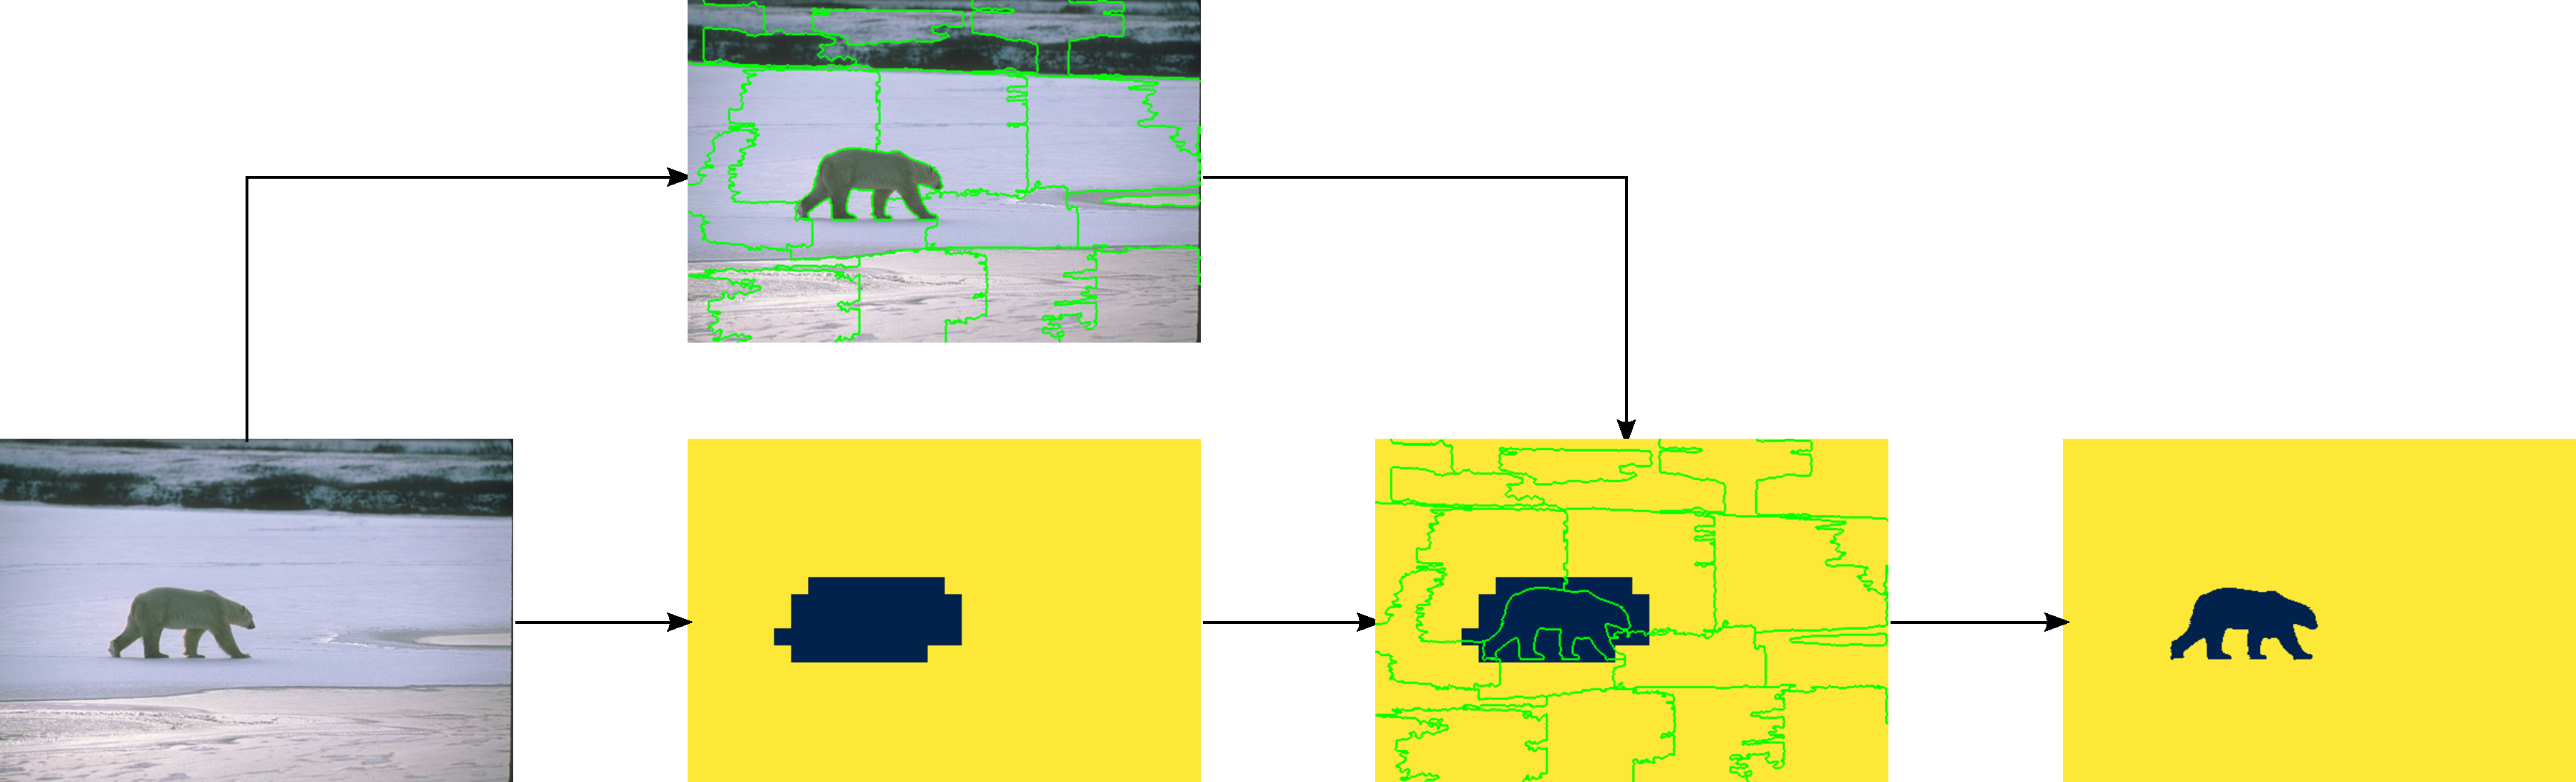
\includegraphics[width=\linewidth]{figures/smv.pdf}
    \caption{An outline of the boundary refinement process. The color superpixel image is superimposed on the segmentation mask. Then, each superpixel is labelled with its majority label.}
    \label{fig:smv}
\end{figure}

In order to use the superpixel image to refine the segmentation mask, both the image and the mask need to have the same spatial resolution. Since more accurate contours are present in the higher resolution superpixel image, the segmentation mask needs to be upsampled. Nearest Neighbour Upsampling can be used to generate the higher resolution mask without introducing new values. Each pixel in the higher resolution mask gets its value from its nearest neighbour pixel in the lower resolution mask.

After upsampling the segmentation mask, the region boundaries can be further refined by employing \emph{Superpixel Majority Voting} (SMV). SMV is a method that uses boundary information from a superpixel color image to correct the region boundaries in a segmentation mask \parencite{feng2021superpixel}. First, SMV superimposes the color superpixel image on the mask. Then, it ensures that all pixels within one superpixel have the same label. It does so by labelling all the pixels within one superpixel by the majority pixel label within that superpixel (see last step in \autoref{fig:smv}). As a result, the jagged edges present in the mask disappear and the regions in the mask adhere well to the boundaries present in the superpixel image.

It is important to note that the size of the superpixels plays an important role in the correction step. Larger superpixels might cover more than one region and yield an image with over-corrected boundaries. This results in parts of the foreground merging with the background. In contrast, smaller superpixels cannot significantly change the contours. This limits the amount of correction made by SMV. Thus, the final contours might be under-corrected.

Another factor that affects the SMV output is the quality of the segmentation mask. SMV cannot correct a poor segmentation mask where the proposed regions are too large compared to the actual size occupied by their corresponding objects. This is due to the error in the poor segmentation mask being enlarged during the upsampling process before applying SMV.